\section{全文总结与展望}
\subsection{全文总结}
    本文提出并实现了一整套完整的基于粒子的流体模拟、渲染、交互系统。其中,流体模拟的关键在于保证不可压缩性求解流体压强,本文将基于位置的动力学(PBD)的思想应用于流体,推导出了基于位置的流体密度约束迭代求解方案。为了进一步完善边界处流体密度欠采样的问题,并实现固液耦合效果,本文采用了边界体积贴图(Volume Map)的隐式SPH边界处理方法。进一步,为了提高流体模拟的真实感,本文在流体压强求解器之后又加入了三种非压强力的求解模型。其次,在工程上,本文采用了空间网格划分加速邻域粒子搜索,并将其完全并行化。另外,本文又提出了一套针对粒子流体模拟结果的屏幕空间实时渲染方法。最后,本文将上述流体仿真方案整合为一套高度并行化的仿真算法,完全使用WebGPU实现。
    
    概况下来,本文的主要工作及贡献包括以下几点:
    
    \begin{enumerate}
    	\item 实现了基于位置的流体模拟方法。传统的SPH方法直接显式计算压强再通过时间积分更新粒子位置,仅能在时间步长很小的情况下才能保持稳定,这会变相降低流体模拟效率,难以应用在实时应用中。而基于位置的流体模拟方法同通过迭代计算密度约束的方法,保证了模拟过程中的流体不可压缩性,支持大时间步模拟。另外,相比于其他迭代求解方法,PBF直接更新粒子位置,没有采用传统的时间积分的方式,进一步简化了求解框架,使得其更适合应用于实时流体模拟。
    	\item 实现了隐式边界条件。粒子法在流体接近于固体边界的部分会由于欠采样而造成流体密度计算出现偏差,需要施加相应的边界条件实现流固耦合。传统的显示边界表示方式将固体边界体素化为粒子,并参与流体粒子的密度计算中。这种方式一方面会由于体素化的离散方式而产生较大误差。另一方面固体粒子也占用过多流体粒子的计算资源,在浏览器环境这种影响更加明显。而本文采用的边界体积方法是一种隐式边界表示方法,它需要将边界体积预计算为一张三维贴图,但是在流体模拟时可以快速查询边界条件对流体粒子的影响,在拥有更高计算精度的同时计算效率更高。
    	\item 通过添加非压强力改善流体细节。首先,由于在压强求解时我们没有考虑负压强的影响,所以本文在非压强力中添加了一个更加物理准确的表面张力模型。一方面在微观视角计算粒子内聚力,另一方面从宏观视角从表面曲率中计算最小化流体表面积的外力。其次,由于数值计算带来的阻尼,流体速度场涡量会快速降低,所以本文增加了一个涡量补偿力像系统中注入能量,保证流体的湍流细节。最后,由于压强解算使用的是密度约束而非速度散度约束,会造成流体速度场存在高频噪声,所以本文增加了人工粘性力,缓解粒子不真实的震荡现象。通过这三种非压强力,本文的流体模拟系统在实时仿真的同时能够保证足够的模拟真实感。
    	\item 实现了并行化的高效粒子搜索算法。临近粒子搜索往往是基于粒子的模拟方法的性能瓶颈。本文通过空间网格划分的方法加速了搜索算法的过程。但是算法中数据依赖性较强,本文使用了计算排序的方法,在不大量引入冗余存储空间的前提下使算法完全并行化。这其中一个重要算法是并行计算数组前缀和,本文采用了两趟遍历二叉树的思想使其并行化,并在具体实现中结合GPU硬件架构,在分支分歧、共享内存、内存Bank冲突等多方面进行优化,提高了粒子搜索的算法性能。
    	\item 实现了高效的屏幕空间流体渲染。在得到模拟结果流体粒子之后,传统的渲染方法往往是从大量粒子中提取表面网格,再将其通过传统的光栅化或光线追踪完成渲染,这在实时应用中显然是不可接受的。本文采用的渲染方法直接将这些流体粒子进行光栅化,不过并不是得到着色结果,而是得到深度和厚度图。然后使用窄域滤波器对深度图进行滤波,相比于双边滤波器,窄域滤波器能完全忽略深度差异过大的采用点之间的互相影响,在得到平滑的深度的同时保留流体边界的深度值突变。最后在屏幕空间完成流体渲染。这种渲染方法可以在保留流体真实感的同时高效执行。
    	\item 使用WebGPU在浏览器环境实现了本文介绍的流体仿真系统。传统的流体仿真由于性能要求,基本都使用C++在本地环境中构建,在跨平台、安装分享、硬件需求方面有着天然的劣势。但是随着新一代浏览器端图形API——WebGPU的发布,在浏览器端调用GPU资源运行流体仿真这种复杂应用遍成为了可能。本文使用了WebGPU实现了流体仿真系统,读者不需要安装任何插件即可浏览体现本流体仿真系统。 
    \\
    \href{https://linzhouli.github.io/WebGPU-Fluid-Simulation/}{https://linzhouli.github.io/WebGPU-Fluid-Simulation/}
    \end{enumerate}

    \begin{figure}[htbp]
    	\centering
    	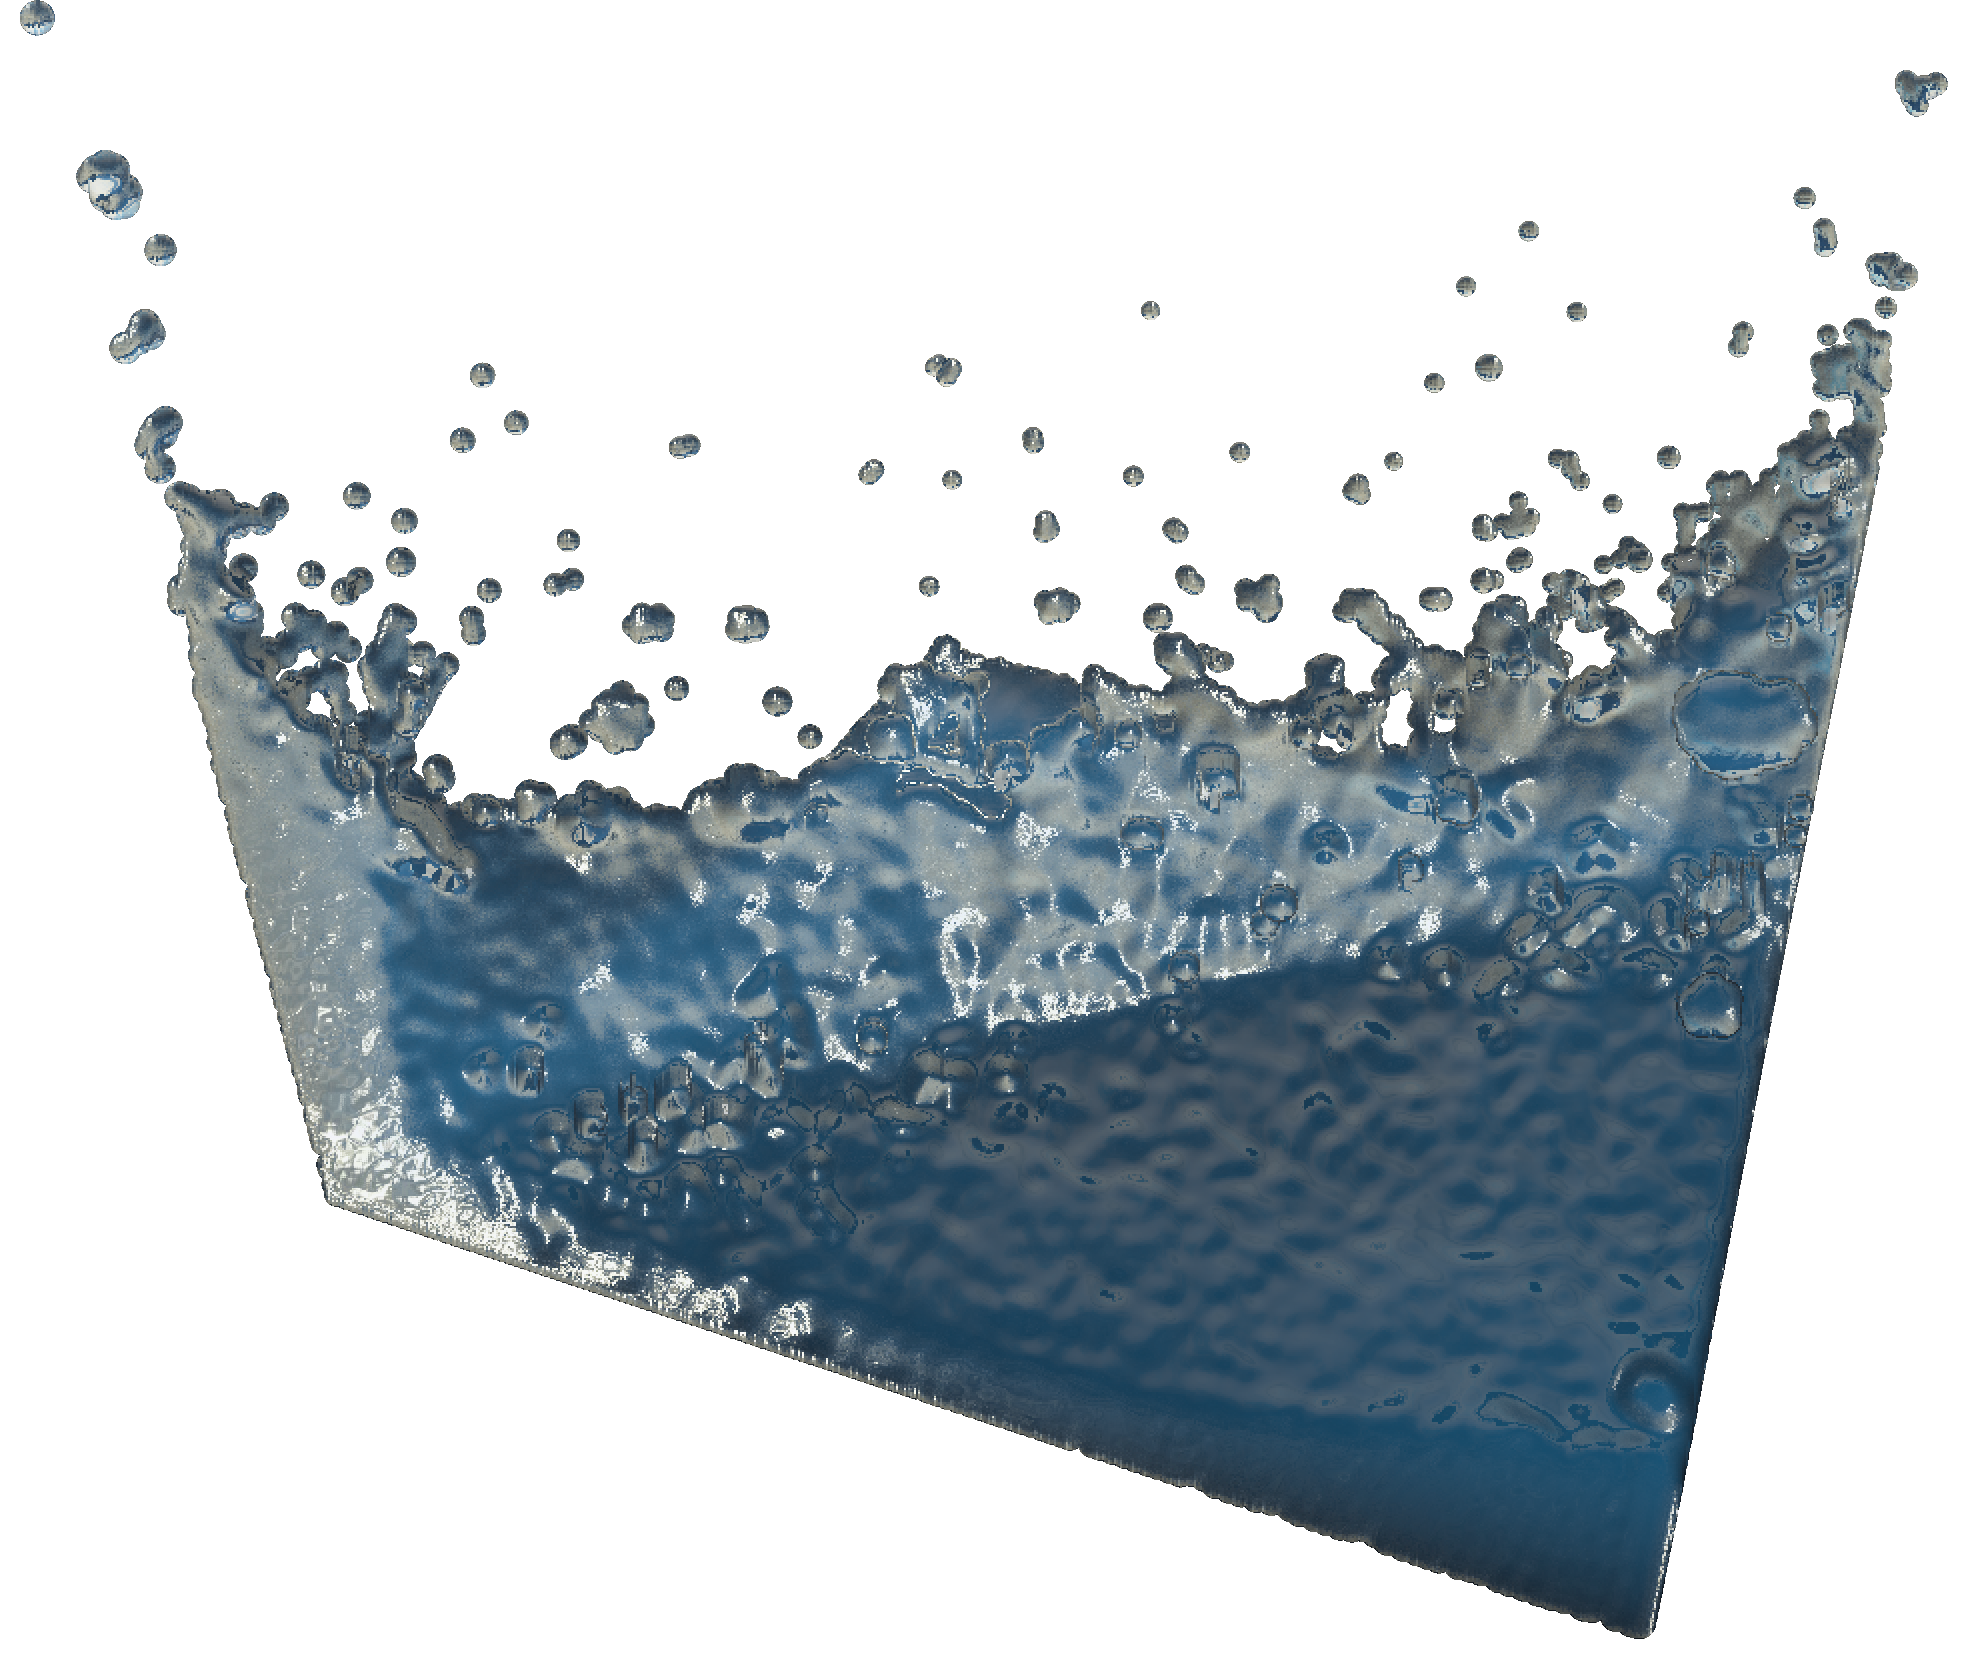
\includegraphics[width=.9\textwidth]{figures/webgpu/result.png}
    	\caption{流体仿真系统}
    \end{figure}

\subsection{存在的不足}
    本文提出的流体仿真系统仍存在许多不足,概况如下:
    
    \begin{enumerate}
    	\item 流体模拟真实感欠佳。在流体压强解算方面,本文实现的PBF框架会仍会造成密度约束求解不充分,流体显得比较“粘滞”,能量耗散较快。在表面张力方面,流体会聚集成团状,难以形成真实的“藕断丝连”的效果,并且本文仅实现了流体粒子之间的内聚力,并没有实现流体与固体之间的黏着力,未能表现出疏水或亲水材质的效果。在流体粘性方面,本文仅采用了简单的显示处理方式,无法表现大粘度流体,比如蜂蜜,酸奶等。
    	\item 流体渲染中,深度图滤波后出现瑕疵。处于性能考虑。本文将深度平滑阶段使用的2D窄域滤波核拆分为两个1D滤波核,分别为X方向和Y方向,但是窄域滤波在数学上并不是可分离的滤波核,这样实现会造成流体轮廓处出现一定瑕疵,在法向还原后会更加严重(如图\ref{fig:dtpn})。这种现象可以通过在两个1D滤波后进行一次小的2D滤波来缓解,但本文并未实现。
    	\item 流体规模较小。由于WebGPU对工作组线程数量的限制,前缀和计算算法最高支持的数组长度也有上限,所以本仿真系统最高支持的流体粒子数量为256K个,相比于本地流体模拟百万级的粒子规模,本仿真系统在仿真细节上有一定缺失。
    	\item 不支持动态边界条件。本文实现的隐式边界条件处理方法仅支持静态物体边界,无法实现双向流固耦合,比如皮球漂浮在水面上随波逐流的效果。
    	\item 邻域粒子查找效率仍有待提高。文本实现的邻域粒子查找方法通过空间划分的结构进行加速,在排序时可以进一步使用网格的z-cureve索引,使得空间上靠近的粒子的物理信息在实际的线性存储空间内也相对靠近,可以大大提高算法的空间局部性,提高缓存命中率。
    \end{enumerate}

\subsection{未来展望}
    本文证明了使用WebGPU在浏览器环境中实现3D复杂流体实时仿真的可行性,并展示了浏览器端流体仿真的广阔应用场景和研究前景。
    
    首先,我们可以将更多高效的GPU并行物理模拟算法移植到浏览器环境中,以充分利用其跨平台优势。例如,布料仿真算法、毛发模拟算法、光线追踪算法等等。
    
    其次,WebGPU流体仿真可以应用于各种实际应用中,例如网页游戏、影视特效、WebVR等。通过实时的复杂3D流体模拟,这些应用可以获得更高的真实感和沉浸感,提升用户体验。
    
    最后,WebGPU为浏览器提供了更底层的GPU计算能力,为在浏览器中运行机器学习模型(WebML)提供更高效的支持。随着ChatGPT引发了下一轮AI热潮,浏览器端也出现了基于WebGPU的大规模模型,例如WebLLM和Web Stable Diffusion。此外,AI在科学领域的应用也正如火如荼,这些条件使得通过深度学习模型加速的Web端流体仿真成为可能。
    
    总之,WebGPU在浏览器端流体仿真的应用为各个领域带来了令人兴奋的可能性,涵盖了娱乐和科学研究等广泛范围。随着网络技术的不断发展和对真实感和交互性体验的需求不断增加,浏览器端流体仿真具备令人期待的未来发展前景。